\documentclass[11pt, letterpaper]{article}

% Fonts and Encoding
\usepackage[utf8]{inputenc}
\usepackage[T1]{fontenc}
\usepackage{lmodern} % High-quality Latin Modern vector font

% Math and Symbols
\usepackage{amsmath, amssymb, amsthm, amsfonts, mathrsfs, mathtools}

% Layout and Geometry
\usepackage{geometry}
\geometry{letterpaper, margin=1in}
\setlength{\parindent}{0pt}
\setlength{\parskip}{0.6em}

% Formatting and Graphics
\usepackage{graphicx, xcolor, enumitem, booktabs, array, tabularx}

% TikZ for Illustrations
\usepackage{tikz}
\usetikzlibrary{arrows.meta, positioning, shapes.geometric, calc, backgrounds, matrix}

% Clickable Links and TOC
\usepackage{hyperref}
\hypersetup{
    colorlinks=true,
    linkcolor=blue,
    filecolor=magenta,      
    urlcolor=cyan,
    pdftitle={Advanced Mathematics Topic},
}

% Theorem Environments
\newtheorem{theorem}{Theorem}[section]
\newtheorem{lemma}[theorem]{Lemma}
\newtheorem{proposition}[theorem]{Proposition}
\newtheorem{corollary}[theorem]{Corollary}
\theoremstyle{definition}
\newtheorem{definition}{Definition}[section]
\newtheorem{axiom}{Axiom}[section]
\newtheorem{example}{Example}[section]
\theoremstyle{remark}
\newtheorem{remark}{Remark}[section]

% Custom Commands (Enforced standard notation)
\newcommand{\R}{\mathbb{R}}
\newcommand{\N}{\mathbb{N}}
\newcommand{\Z}{\mathbb{Z}}
\newcommand{\Q}{\mathbb{Q}}
\newcommand{\E}{\mathbb{E}}
\newcommand{\Prob}{\mathbb{P}}
\newcommand{\F}{\mathcal{F}}

\title{Mastering Orthogonal Projections and the Gram-Schmidt Process}
\author{Tashfeen Omran}
\date{\today}

\begin{document}

\maketitle
\tableofcontents
\newpage

\section{Part 1: Comprehensive Introduction, Context, and Prerequisites}

\subsection{Core Concepts}
The topic of \textbf{Orthogonal Projections} lies at the heart of linear algebra and its applications. When we have a vector $\mathbf{y}$ in $\R^n$ and a subspace $W$, we often want to decompose $\mathbf{y}$ into two distinct parts: one part that lies entirely within $W$, and another part that is completely perpendicular (orthogonal) to $W$. 

This is formalized by the \textbf{Orthogonal Decomposition Theorem}, which states that any vector $\mathbf{y} \in \R^n$ can be written uniquely as:
\[ \mathbf{y} = \hat{\mathbf{y}} + \mathbf{z} \]
where $\hat{\mathbf{y}}$ is in $W$ (this is the orthogonal projection of $\mathbf{y}$ onto $W$, denoted $\text{proj}_W \mathbf{y}$) and $\mathbf{z}$ is in $W^\perp$ (the orthogonal complement of $W$). 

Furthermore, the \textbf{Best Approximation Theorem} tells us that $\hat{\mathbf{y}}$ is the closest point in $W$ to $\mathbf{y}$. The distance from $\mathbf{y}$ to the subspace $W$ is exactly the length of the error vector, $\|\mathbf{z}\| = \|\mathbf{y} - \hat{\mathbf{y}}\|$.

\subsection{Intuition and Derivation}
Imagine shining a flashlight directly down onto an object hovering above a flat table. The shadow cast on the table represents the orthogonal projection ($\hat{\mathbf{y}}$). The table itself is the subspace $W$. The invisible vertical line connecting the object to its shadow is the orthogonal error vector ($\mathbf{z}$). 

Mathematically, if we have an orthogonal basis $\{\mathbf{u}_1, \dots, \mathbf{u}_p\}$ for $W$, we can project $\mathbf{y}$ onto each basis vector individually and sum the results. This works \textit{only} because the basis vectors are mutually perpendicular, meaning their individual 1-dimensional shadows do not overlap or interfere with one another.

\subsection{Historical Context and Motivation}
The mathematical machinery of orthogonal projections was heavily developed in the late 18th and early 19th centuries by Carl Friedrich Gauss and Adrien-Marie Legendre. They were attempting to predict the orbits of celestial bodies (like the asteroid Ceres) using astronomical observations that contained measurement errors. They needed a way to find the "best fit" line or curve through noisy data. This led to the Method of Least Squares, which is fundamentally an application of orthogonal projection: projecting a vector of observed data onto the column space of a matrix to minimize the squared error.

\subsection{Key Formulas}
\begin{itemize}
    \item \textbf{Orthogonal Projection Formula:} If $\{\mathbf{u}_1, \dots, \mathbf{u}_p\}$ is an \textit{orthogonal} basis for $W$, then:
    \[ \hat{\mathbf{y}} = \text{proj}_W \mathbf{y} = \frac{\mathbf{y} \cdot \mathbf{u}_1}{\mathbf{u}_1 \cdot \mathbf{u}_1}\mathbf{u}_1 + \frac{\mathbf{y} \cdot \mathbf{u}_2}{\mathbf{u}_2 \cdot \mathbf{u}_2}\mathbf{u}_2 + \dots + \frac{\mathbf{y} \cdot \mathbf{u}_p}{\mathbf{u}_p \cdot \mathbf{u}_p}\mathbf{u}_p \]
    \item \textbf{Orthogonal Error Vector:} 
    \[ \mathbf{z} = \mathbf{y} - \hat{\mathbf{y}} \]
    \item \textbf{Distance to a Subspace:} 
    \[ \text{Distance} = \|\mathbf{y} - \hat{\mathbf{y}}\| = \sqrt{\mathbf{z} \cdot \mathbf{z}} \]
    \item \textbf{Projection via Orthonormal Matrix:} If $U$ is a matrix whose columns form an \textit{orthonormal} basis for $W$, then:
    \[ \text{proj}_W \mathbf{y} = U U^T \mathbf{y} \]
\end{itemize}

\subsection{Prerequisites}
To succeed in this topic, you must be fluent in:
\begin{enumerate}
    \item \textbf{Dot Products:} Computing $\mathbf{u} \cdot \mathbf{v} = u_1v_1 + \dots + u_nv_n$.
    \item \textbf{Vector Norms:} Calculating the length of a vector $\|\mathbf{v}\| = \sqrt{\mathbf{v} \cdot \mathbf{v}}$.
    \item \textbf{Subspaces and Bases:} Understanding what it means for a set of vectors to span a space and be linearly independent.
    \item \textbf{Matrix Multiplication and Transposes:} Computing $U^T U$ and $U U^T$.
\end{enumerate}

\newpage
\section{Part 2: Detailed Homework Solutions}

\textit{Note: To maximize learning efficiency and avoid redundant repetition, a strategic selection of problems has been chosen. This sample covers at least two of every distinct problem archetype found in the text.}

\subsection{Problem 3: Verifying Orthogonality and Finding Projections}
\textbf{Original Problem:} Verify that $\{\mathbf{u}_1, \mathbf{u}_2\}$ is an orthogonal set, and then find the orthogonal projection of $\mathbf{y}$ onto $\text{Span}\{\mathbf{u}_1, \mathbf{u}_2\}$.
\[ \mathbf{y} = \begin{bmatrix} -1 \\ 4 \\ 3 \end{bmatrix}, \quad \mathbf{u}_1 = \begin{bmatrix} 1 \\ 1 \\ 0 \end{bmatrix}, \quad \mathbf{u}_2 = \begin{bmatrix} -1 \\ 1 \\ 0 \end{bmatrix} \]

\textbf{Solution:}
\textbf{Step 1: Verify orthogonality.}
We must show that the dot product $\mathbf{u}_1 \cdot \mathbf{u}_2 = 0$.
\[ \mathbf{u}_1 \cdot \mathbf{u}_2 = (1)(-1) + (1)(1) + (0)(0) = -1 + 1 + 0 = 0 \]
Since the dot product is zero, the set is orthogonal.

\textbf{Step 2: Compute the orthogonal projection.}
Since the basis is orthogonal, we use the projection formula:
\[ \hat{\mathbf{y}} = \frac{\mathbf{y} \cdot \mathbf{u}_1}{\mathbf{u}_1 \cdot \mathbf{u}_1}\mathbf{u}_1 + \frac{\mathbf{y} \cdot \mathbf{u}_2}{\mathbf{u}_2 \cdot \mathbf{u}_2}\mathbf{u}_2 \]
First, compute the necessary dot products:
\begin{align*}
    \mathbf{y} \cdot \mathbf{u}_1 &= (-1)(1) + (4)(1) + (3)(0) = 3 \\
    \mathbf{u}_1 \cdot \mathbf{u}_1 &= (1)^2 + (1)^2 + (0)^2 = 2 \\
    \mathbf{y} \cdot \mathbf{u}_2 &= (-1)(-1) + (4)(1) + (3)(0) = 5 \\
    \mathbf{u}_2 \cdot \mathbf{u}_2 &= (-1)^2 + (1)^2 + (0)^2 = 2
\end{align*}
Now, substitute these values into the formula:
\[ \hat{\mathbf{y}} = \frac{3}{2} \begin{bmatrix} 1 \\ 1 \\ 0 \end{bmatrix} + \frac{5}{2} \begin{bmatrix} -1 \\ 1 \\ 0 \end{bmatrix} = \begin{bmatrix} 3/2 \\ 3/2 \\ 0 \end{bmatrix} + \begin{bmatrix} -5/2 \\ 5/2 \\ 0 \end{bmatrix} = \begin{bmatrix} -2/2 \\ 8/2 \\ 0 \end{bmatrix} = \begin{bmatrix} -1 \\ 4 \\ 0 \end{bmatrix} \]

\textbf{Final Answer:} $\hat{\mathbf{y}} = \begin{bmatrix} -1 \\ 4 \\ 0 \end{bmatrix}$

\vspace{1em}
\subsection{Problem 5: Verifying Orthogonality and Finding Projections}
\textbf{Original Problem:} Verify that $\{\mathbf{u}_1, \mathbf{u}_2\}$ is an orthogonal set, and then find the orthogonal projection of $\mathbf{y}$ onto $\text{Span}\{\mathbf{u}_1, \mathbf{u}_2\}$.
\[ \mathbf{y} = \begin{bmatrix} -1 \\ 2 \\ 6 \end{bmatrix}, \quad \mathbf{u}_1 = \begin{bmatrix} 3 \\ -1 \\ 2 \end{bmatrix}, \quad \mathbf{u}_2 = \begin{bmatrix} 1 \\ -1 \\ -2 \end{bmatrix} \]

\textbf{Solution:}
\textbf{Step 1: Verify orthogonality.}
\[ \mathbf{u}_1 \cdot \mathbf{u}_2 = (3)(1) + (-1)(-1) + (2)(-2) = 3 + 1 - 4 = 0 \]
The set is orthogonal.

\textbf{Step 2: Compute the orthogonal projection.}
\begin{align*}
    \mathbf{y} \cdot \mathbf{u}_1 &= (-1)(3) + (2)(-1) + (6)(2) = -3 - 2 + 12 = 7 \\
    \mathbf{u}_1 \cdot \mathbf{u}_1 &= (3)^2 + (-1)^2 + (2)^2 = 9 + 1 + 4 = 14 \\
    \mathbf{y} \cdot \mathbf{u}_2 &= (-1)(1) + (2)(-1) + (6)(-2) = -1 - 2 - 12 = -15 \\
    \mathbf{u}_2 \cdot \mathbf{u}_2 &= (1)^2 + (-1)^2 + (-2)^2 = 1 + 1 + 4 = 6
\end{align*}
Substitute into the projection formula:
\[ \hat{\mathbf{y}} = \frac{7}{14} \begin{bmatrix} 3 \\ -1 \\ 2 \end{bmatrix} + \frac{-15}{6} \begin{bmatrix} 1 \\ -1 \\ -2 \end{bmatrix} = \frac{1}{2} \begin{bmatrix} 3 \\ -1 \\ 2 \end{bmatrix} - \frac{5}{2} \begin{bmatrix} 1 \\ -1 \\ -2 \end{bmatrix} \]
\[ \hat{\mathbf{y}} = \begin{bmatrix} 3/2 \\ -1/2 \\ 1 \end{bmatrix} - \begin{bmatrix} 5/2 \\ -5/2 \\ -5 \end{bmatrix} = \begin{bmatrix} -2/2 \\ 4/2 \\ 6 \end{bmatrix} = \begin{bmatrix} -1 \\ 2 \\ 6 \end{bmatrix} \]
\textit{Remark: Because $\hat{\mathbf{y}} = \mathbf{y}$, this implies that $\mathbf{y}$ was already in the subspace spanned by $\mathbf{u}_1$ and $\mathbf{u}_2$.}

\textbf{Final Answer:} $\hat{\mathbf{y}} = \begin{bmatrix} -1 \\ 2 \\ 6 \end{bmatrix}$

\vspace{1em}
\subsection{Problem 7: Orthogonal Decomposition}
\textbf{Original Problem:} Let $W$ be the subspace spanned by the $\mathbf{u}$'s, and write $\mathbf{y}$ as the sum of a vector in $W$ and a vector orthogonal to $W$.
\[ \mathbf{y} = \begin{bmatrix} 1 \\ 3 \\ 5 \end{bmatrix}, \quad \mathbf{u}_1 = \begin{bmatrix} 1 \\ 3 \\ -2 \end{bmatrix}, \quad \mathbf{u}_2 = \begin{bmatrix} 5 \\ 1 \\ 4 \end{bmatrix} \]

\textbf{Solution:}
\textbf{Step 1: Verify the basis is orthogonal.}
\[ \mathbf{u}_1 \cdot \mathbf{u}_2 = (1)(5) + (3)(1) + (-2)(4) = 5 + 3 - 8 = 0 \]

\textbf{Step 2: Find $\hat{\mathbf{y}}$ (the vector in $W$).}
\begin{align*}
    \mathbf{y} \cdot \mathbf{u}_1 &= (1)(1) + (3)(3) + (5)(-2) = 1 + 9 - 10 = 0 \\
    \mathbf{u}_1 \cdot \mathbf{u}_1 &= 1^2 + 3^2 + (-2)^2 = 1 + 9 + 4 = 14 \\
    \mathbf{y} \cdot \mathbf{u}_2 &= (1)(5) + (3)(1) + (5)(4) = 5 + 3 + 20 = 28 \\
    \mathbf{u}_2 \cdot \mathbf{u}_2 &= 5^2 + 1^2 + 4^2 = 25 + 1 + 16 = 42
\end{align*}
\[ \hat{\mathbf{y}} = \frac{0}{14}\mathbf{u}_1 + \frac{28}{42}\mathbf{u}_2 = 0 + \frac{2}{3} \begin{bmatrix} 5 \\ 1 \\ 4 \end{bmatrix} = \begin{bmatrix} 10/3 \\ 2/3 \\ 8/3 \end{bmatrix} \]

\textbf{Step 3: Find $\mathbf{z}$ (the vector orthogonal to $W$).}
\[ \mathbf{z} = \mathbf{y} - \hat{\mathbf{y}} = \begin{bmatrix} 1 \\ 3 \\ 5 \end{bmatrix} - \begin{bmatrix} 10/3 \\ 2/3 \\ 8/3 \end{bmatrix} = \begin{bmatrix} 3/3 - 10/3 \\ 9/3 - 2/3 \\ 15/3 - 8/3 \end{bmatrix} = \begin{bmatrix} -7/3 \\ 7/3 \\ 7/3 \end{bmatrix} \]

\textbf{Final Answer:} $\mathbf{y} = \begin{bmatrix} 10/3 \\ 2/3 \\ 8/3 \end{bmatrix} + \begin{bmatrix} -7/3 \\ 7/3 \\ 7/3 \end{bmatrix}$

\vspace{1em}
\subsection{Problem 11: Best Approximation}
\textbf{Original Problem:} Find the closest point to $\mathbf{y}$ in the subspace $W$ spanned by $\mathbf{v}_1$ and $\mathbf{v}_2$.
\[ \mathbf{y} = \begin{bmatrix} 3 \\ 1 \\ 5 \\ 1 \end{bmatrix}, \quad \mathbf{v}_1 = \begin{bmatrix} 3 \\ 1 \\ -1 \\ 1 \end{bmatrix}, \quad \mathbf{v}_2 = \begin{bmatrix} 1 \\ -1 \\ 1 \\ -1 \end{bmatrix} \]

\textbf{Solution:}
By the Best Approximation Theorem, the closest point in $W$ to $\mathbf{y}$ is the orthogonal projection $\hat{\mathbf{y}}$.
\textbf{Step 1: Verify orthogonality of the basis.}
\[ \mathbf{v}_1 \cdot \mathbf{v}_2 = (3)(1) + (1)(-1) + (-1)(1) + (1)(-1) = 3 - 1 - 1 - 1 = 0 \]

\textbf{Step 2: Compute the projection.}
\begin{align*}
    \mathbf{y} \cdot \mathbf{v}_1 &= 9 + 1 - 5 + 1 = 6 \\
    \mathbf{v}_1 \cdot \mathbf{v}_1 &= 9 + 1 + 1 + 1 = 12 \\
    \mathbf{y} \cdot \mathbf{v}_2 &= 3 - 1 + 5 - 1 = 6 \\
    \mathbf{v}_2 \cdot \mathbf{v}_2 &= 1 + 1 + 1 + 1 = 4
\end{align*}
\[ \hat{\mathbf{y}} = \frac{6}{12}\mathbf{v}_1 + \frac{6}{4}\mathbf{v}_2 = \frac{1}{2} \begin{bmatrix} 3 \\ 1 \\ -1 \\ 1 \end{bmatrix} + \frac{3}{2} \begin{bmatrix} 1 \\ -1 \\ 1 \\ -1 \end{bmatrix} = \begin{bmatrix} 3/2 + 3/2 \\ 1/2 - 3/2 \\ -1/2 + 3/2 \\ 1/2 - 3/2 \end{bmatrix} = \begin{bmatrix} 3 \\ -1 \\ 1 \\ -1 \end{bmatrix} \]

\textbf{Final Answer:} The closest point is $\begin{bmatrix} 3 \\ -1 \\ 1 \\ -1 \end{bmatrix}$.

\vspace{1em}
\subsection{Problem 15: Distance to a Subspace}
\textbf{Original Problem:} Find the distance from $\mathbf{y}$ to the plane in $\R^3$ spanned by $\mathbf{u}_1$ and $\mathbf{u}_2$.
\[ \mathbf{y} = \begin{bmatrix} 5 \\ -9 \\ 5 \end{bmatrix}, \quad \mathbf{u}_1 = \begin{bmatrix} -3 \\ -5 \\ 1 \end{bmatrix}, \quad \mathbf{u}_2 = \begin{bmatrix} -3 \\ 2 \\ 1 \end{bmatrix} \]

\textbf{Solution:}
The distance is given by $\|\mathbf{z}\| = \|\mathbf{y} - \hat{\mathbf{y}}\|$.
\textbf{Step 1: Verify orthogonality.}
\[ \mathbf{u}_1 \cdot \mathbf{u}_2 = (-3)(-3) + (-5)(2) + (1)(1) = 9 - 10 + 1 = 0 \]

\textbf{Step 2: Compute $\hat{\mathbf{y}}$.}
\begin{align*}
    \mathbf{y} \cdot \mathbf{u}_1 &= -15 + 45 + 5 = 35 \\
    \mathbf{u}_1 \cdot \mathbf{u}_1 &= 9 + 25 + 1 = 35 \\
    \mathbf{y} \cdot \mathbf{u}_2 &= -15 - 18 + 5 = -28 \\
    \mathbf{u}_2 \cdot \mathbf{u}_2 &= 9 + 4 + 1 = 14
\end{align*}
\[ \hat{\mathbf{y}} = \frac{35}{35}\mathbf{u}_1 - \frac{28}{14}\mathbf{u}_2 = 1\begin{bmatrix} -3 \\ -5 \\ 1 \end{bmatrix} - 2\begin{bmatrix} -3 \\ 2 \\ 1 \end{bmatrix} = \begin{bmatrix} -3 + 6 \\ -5 - 4 \\ 1 - 2 \end{bmatrix} = \begin{bmatrix} 3 \\ -9 \\ -1 \end{bmatrix} \]

\textbf{Step 3: Compute $\mathbf{z}$ and its norm.}
\[ \mathbf{z} = \mathbf{y} - \hat{\mathbf{y}} = \begin{bmatrix} 5 \\ -9 \\ 5 \end{bmatrix} - \begin{bmatrix} 3 \\ -9 \\ -1 \end{bmatrix} = \begin{bmatrix} 2 \\ 0 \\ 6 \end{bmatrix} \]
\[ \|\mathbf{z}\| = \sqrt{2^2 + 0^2 + 6^2} = \sqrt{4 + 36} = \sqrt{40} = 2\sqrt{10} \]

\textbf{Final Answer:} The distance is $2\sqrt{10}$.

\vspace{1em}
\subsection{Problem 17: Orthonormal Matrices}
\textbf{Original Problem:} Let $\mathbf{y} = \begin{bmatrix} 4 \\ 8 \\ 1 \end{bmatrix}$, $\mathbf{u}_1 = \begin{bmatrix} 2/3 \\ 1/3 \\ 2/3 \end{bmatrix}$, $\mathbf{u}_2 = \begin{bmatrix} -2/3 \\ 2/3 \\ 1/3 \end{bmatrix}$, and $W = \text{Span}\{\mathbf{u}_1, \mathbf{u}_2\}$.
a. Let $U = [\mathbf{u}_1 \quad \mathbf{u}_2]$. Compute $U^T U$ and $U U^T$.
b. Compute $\text{proj}_W \mathbf{y}$ and $(U U^T)\mathbf{y}$.

\textbf{Solution:}
\textbf{Part a:}
\[ U = \begin{bmatrix} 2/3 & -2/3 \\ 1/3 & 2/3 \\ 2/3 & 1/3 \end{bmatrix}, \quad U^T = \begin{bmatrix} 2/3 & 1/3 & 2/3 \\ -2/3 & 2/3 & 1/3 \end{bmatrix} \]
\[ U^T U = \begin{bmatrix} 2/3 & 1/3 & 2/3 \\ -2/3 & 2/3 & 1/3 \end{bmatrix} \begin{bmatrix} 2/3 & -2/3 \\ 1/3 & 2/3 \\ 2/3 & 1/3 \end{bmatrix} = \begin{bmatrix} \frac{4+1+4}{9} & \frac{-4+2+2}{9} \\ \frac{-4+2+2}{9} & \frac{4+4+1}{9} \end{bmatrix} = \begin{bmatrix} 1 & 0 \\ 0 & 1 \end{bmatrix} \]
\[ U U^T = \begin{bmatrix} 2/3 & -2/3 \\ 1/3 & 2/3 \\ 2/3 & 1/3 \end{bmatrix} \begin{bmatrix} 2/3 & 1/3 & 2/3 \\ -2/3 & 2/3 & 1/3 \end{bmatrix} = \begin{bmatrix} 8/9 & -2/9 & 2/9 \\ -2/9 & 5/9 & 4/9 \\ 2/9 & 4/9 & 5/9 \end{bmatrix} \]

\textbf{Part b:}
Using the standard projection formula:
\begin{align*}
    \mathbf{y} \cdot \mathbf{u}_1 &= 8/3 + 8/3 + 2/3 = 18/3 = 6 \\
    \mathbf{y} \cdot \mathbf{u}_2 &= -8/3 + 16/3 + 1/3 = 9/3 = 3
\end{align*}
(Note: denominators are 1 because the basis is orthonormal).
\[ \text{proj}_W \mathbf{y} = 6\begin{bmatrix} 2/3 \\ 1/3 \\ 2/3 \end{bmatrix} + 3\begin{bmatrix} -2/3 \\ 2/3 \\ 1/3 \end{bmatrix} = \begin{bmatrix} 4 \\ 2 \\ 4 \end{bmatrix} + \begin{bmatrix} -2 \\ 2 \\ 1 \end{bmatrix} = \begin{bmatrix} 2 \\ 4 \\ 5 \end{bmatrix} \]
Now using the matrix formula:
\[ (U U^T)\mathbf{y} = \begin{bmatrix} 8/9 & -2/9 & 2/9 \\ -2/9 & 5/9 & 4/9 \\ 2/9 & 4/9 & 5/9 \end{bmatrix} \begin{bmatrix} 4 \\ 8 \\ 1 \end{bmatrix} = \begin{bmatrix} 32/9 - 16/9 + 2/9 \\ -8/9 + 40/9 + 4/9 \\ 8/9 + 32/9 + 5/9 \end{bmatrix} = \begin{bmatrix} 18/9 \\ 36/9 \\ 45/9 \end{bmatrix} = \begin{bmatrix} 2 \\ 4 \\ 5 \end{bmatrix} \]

\textbf{Final Answer:} 
a. $U^T U = \begin{bmatrix} 1 & 0 \\ 0 & 1 \end{bmatrix}$, $U U^T = \begin{bmatrix} 8/9 & -2/9 & 2/9 \\ -2/9 & 5/9 & 4/9 \\ 2/9 & 4/9 & 5/9 \end{bmatrix}$. 
b. Both yield $\begin{bmatrix} 2 \\ 4 \\ 5 \end{bmatrix}$.

\vspace{1em}
\subsection{Problems 21 \& 22: Conceptual True/False}
\textbf{Problem 21:} (T/F) If $\mathbf{z}$ is orthogonal to $\mathbf{u}_1$ and to $\mathbf{u}_2$ and if $W = \text{Span}\{\mathbf{u}_1, \mathbf{u}_2\}$, then $\mathbf{z}$ must be in $W^\perp$.
\textbf{Solution:} \textbf{True.} If a vector is orthogonal to every vector in a basis for $W$, it is orthogonal to every linear combination of those basis vectors, and thus orthogonal to all of $W$.

\textbf{Problem 22:} (T/F) For each $\mathbf{y}$ and each subspace $W$, the vector $\mathbf{y} - \text{proj}_W \mathbf{y}$ is orthogonal to $W$.
\textbf{Solution:} \textbf{True.} By the Orthogonal Decomposition Theorem, $\mathbf{y} = \hat{\mathbf{y}} + \mathbf{z}$, where $\hat{\mathbf{y}} = \text{proj}_W \mathbf{y}$ and $\mathbf{z} \in W^\perp$. Rearranging gives $\mathbf{z} = \mathbf{y} - \text{proj}_W \mathbf{y}$, which is in $W^\perp$.

\newpage
\section{Part 3: In-Depth Analysis of Problems and Techniques}

\subsection{A) Problem Types and General Approach}
\begin{itemize}
    \item \textbf{Type 1: Verification and Projection (Problems 3, 5):} 
    \textit{Approach:} Always begin by taking the dot product of the basis vectors to ensure they equal zero. If they do, apply the standard projection formula. If they do not, the formula will fail (requiring Gram-Schmidt first).
    \item \textbf{Type 2: Orthogonal Decomposition (Problem 7):} 
    \textit{Approach:} This is a two-step process. First, find $\hat{\mathbf{y}}$ using the projection formula. Second, use vector subtraction $\mathbf{z} = \mathbf{y} - \hat{\mathbf{y}}$ to find the orthogonal component.
    \item \textbf{Type 3: Best Approximation and Distance (Problems 11, 15):} 
    \textit{Approach:} Recognize that "closest point" and "best approximation" are synonyms for the orthogonal projection $\hat{\mathbf{y}}$. "Distance" is the magnitude of the error vector, $\|\mathbf{y} - \hat{\mathbf{y}}\|$.
    \item \textbf{Type 4: Orthonormal Matrices (Problem 17):} 
    \textit{Approach:} Recognize that if columns are orthonormal, $U^T U = I$. The projection matrix onto the column space is $U U^T$. This is computationally faster than the standard formula because all denominators ($\mathbf{u}_i \cdot \mathbf{u}_i$) are exactly 1.
\end{itemize}

\subsection{B) Key Algebraic and Calculus Manipulations}
\begin{itemize}
    \item \textbf{The Zero-Check Sanity Trick:} In Problem 7, after calculating $\mathbf{z} = \begin{bmatrix} -7/3 \\ 7/3 \\ 7/3 \end{bmatrix}$, a crucial algebraic manipulation is to mentally dot $\mathbf{z}$ with $\mathbf{u}_1$. $(-7/3)(1) + (7/3)(3) + (7/3)(-2) = -7/3 + 21/3 - 14/3 = 0$. This instantly verifies that the arithmetic for the entire problem is correct.
    \item \textbf{Factoring out Scalars:} In Problem 15, the projection yielded $\frac{35}{35}\mathbf{u}_1 - \frac{28}{14}\mathbf{u}_2$. Simplifying the fractions \textit{before} distributing them into the vectors prevents messy fraction arithmetic.
    \item \textbf{Matrix Multiplication as Projection:} In Problem 17, computing $(U U^T)\mathbf{y}$ demonstrates associativity. It is often easier to compute $U(U^T \mathbf{y})$ than to compute the full $3 \times 3$ matrix $U U^T$ first.
\end{itemize}

\newpage
\section{Part 4: "Cheatsheet" and Tips for Success}

\renewcommand{\arraystretch}{1.5}
\begin{tabularx}{\textwidth}{>{\raggedright\arraybackslash}p{4cm} X}
\toprule
\textbf{Concept} & \textbf{Formula / Rule} \\
\midrule
\textbf{Orthogonal Projection} & $\displaystyle \hat{\mathbf{y}} = \frac{\mathbf{y} \cdot \mathbf{u}_1}{\mathbf{u}_1 \cdot \mathbf{u}_1}\mathbf{u}_1 + \dots + \frac{\mathbf{y} \cdot \mathbf{u}_p}{\mathbf{u}_p \cdot \mathbf{u}_p}\mathbf{u}_p$ \\
\addlinespace[4pt]
\textbf{Error Vector} & $\displaystyle \mathbf{z} = \mathbf{y} - \hat{\mathbf{y}}$ \quad (Always check that $\mathbf{z} \cdot \mathbf{u}_i = 0$) \\
\addlinespace[4pt]
\textbf{Distance to Subspace} & $\displaystyle \|\mathbf{z}\| = \sqrt{\mathbf{z} \cdot \mathbf{z}}$ \\
\addlinespace[4pt]
\textbf{Orthonormal Basis} & If $\|\mathbf{u}_i\| = 1$, the formula simplifies to: $\displaystyle \hat{\mathbf{y}} = (\mathbf{y} \cdot \mathbf{u}_1)\mathbf{u}_1 + \dots + (\mathbf{y} \cdot \mathbf{u}_p)\mathbf{u}_p$ \\
\addlinespace[4pt]
\textbf{Projection Matrix} & If $U$ has orthonormal columns, $\text{proj}_W \mathbf{y} = U U^T \mathbf{y}$. \\
\bottomrule
\end{tabularx}

\vspace{1em}
\textbf{Tips and Pitfalls:}
\begin{itemize}
    \item \textbf{The Non-Orthogonal Trap:} The most common fatal error on exams is applying the projection formula when the basis vectors are \textit{not} orthogonal. Always check $\mathbf{u}_1 \cdot \mathbf{u}_2 = 0$ first. If they aren't orthogonal, you must use the Gram-Schmidt process first.
    \item \textbf{Distance vs. Closest Point:} Read the question carefully. If it asks for the "closest point," the answer is a vector ($\hat{\mathbf{y}}$). If it asks for "distance," the answer is a scalar ($\|\mathbf{y} - \hat{\mathbf{y}}\|$).
    \item \textbf{The $U^T U$ vs $U U^T$ Confusion:} For a non-square matrix $U$ with orthonormal columns, $U^T U$ is the Identity matrix ($I$). However, $U U^T$ is \textit{not} the Identity matrix; it is the Projection matrix onto the column space of $U$.
\end{itemize}

\begin{center}
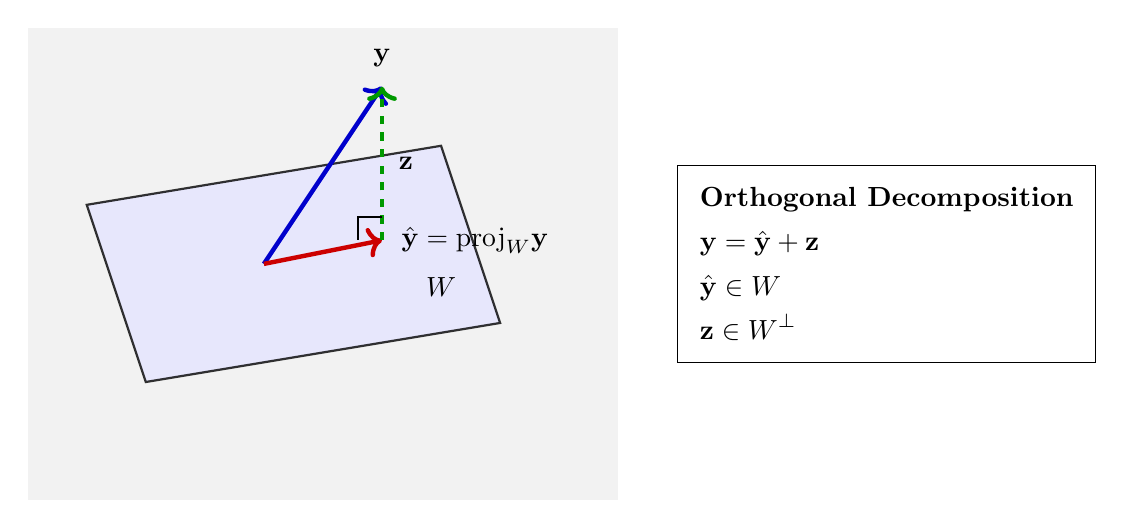
\begin{tikzpicture}[scale=1.5]
    % Background/Grid
    \fill[gray!10] (-1,-1) rectangle (4,3);
    
    % Subspace W (Plane)
    \draw[fill=blue!10, opacity=0.8, thick] (0,0) -- (3,0.5) -- (2.5, 2) -- (-0.5, 1.5) -- cycle;
    \node[black] at (2.5, 0.8) {$W$};
    
    % Vectors
    \draw[->, ultra thick, blue!80!black] (1, 1) -- (2, 2.5) node[above=3pt, black] {$\displaystyle \mathbf{y}$};
    \draw[->, ultra thick, red!80!black] (1, 1) -- (2, 1.2) node[right=3pt, black] {$\displaystyle \hat{\mathbf{y}} = \text{proj}_W \mathbf{y}$};
    \draw[->, ultra thick, dashed, green!60!black] (2, 1.2) -- (2, 2.5) node[midway, right=2pt, black] {$\displaystyle \mathbf{z}$};
    
    % Right angle
    \draw[thick] (2, 1.4) -- (1.8, 1.4) -- (1.8, 1.2);
    
    % Legend
    \node[align=left, fill=white, draw=black, inner sep=8pt, anchor=west] at (4.5, 1) {
        \textbf{Orthogonal Decomposition}\\[4pt]
        $\displaystyle \mathbf{y} = \hat{\mathbf{y}} + \mathbf{z}$\\[4pt]
        $\displaystyle \hat{\mathbf{y}} \in W$\\[4pt]
        $\displaystyle \mathbf{z} \in W^\perp$
    };
\end{tikzpicture}
\end{center}

\newpage
\section{Part 5: Conceptual Synthesis and The "Big Picture"}

\subsection{A) Thematic Connections}
The core theme of this topic is \textbf{Information Compression and Error Minimization}. In mathematics, we frequently encounter vectors (or functions, or data points) that exist in a highly complex, high-dimensional space. We often want to approximate this complex object using a simpler, lower-dimensional space (the subspace $W$). 

Orthogonal projection is the mathematical equivalent of dropping a perpendicular line to find the shortest path. It guarantees that the "shadow" we cast onto the simpler space retains as much of the original information as possible, while the discarded information (the orthogonal error $\mathbf{z}$) is minimized. This exact theme appears in Calculus when we use Taylor Series to approximate complex functions with simpler polynomials.

\subsection{B) Forward and Backward Links}
\textbf{Backward Links:} This topic is the logical culmination of the dot product. Previously, the dot product was just a tool to find angles between vectors. Here, it becomes the engine for decomposing spaces.

\textbf{Forward Links:} Understanding orthogonal projections is the absolute bedrock for:
\begin{itemize}
    \item \textbf{Least Squares Regression:} In statistics, when a system $A\mathbf{x} = \mathbf{b}$ has no solution (because $\mathbf{b}$ is not in the column space of $A$), we project $\mathbf{b}$ onto $\text{Col}(A)$ to find the best possible approximation.
    \item \textbf{Fourier Series:} In differential equations, projecting a continuous function onto an orthogonal basis of sine and cosine waves allows us to decompose sound and light into frequencies.
    \item \textbf{Principal Component Analysis (PCA):} In data science, we project massive datasets onto the eigenvectors of a covariance matrix to reduce dimensionality while preserving variance.
\end{itemize}

\section{Part 6: Abstract Real-World Modeling (AI, ML, \& Quant Finance)}

\subsection{A) Concrete Scenarios}
\begin{enumerate}
    \item \textbf{Quantitative Finance (Arbitrage Pricing Theory):} In multi-factor risk models, a portfolio's return vector is projected onto a subspace spanned by macroeconomic factors (e.g., inflation, market risk, interest rates). The orthogonal component represents the portfolio's idiosyncratic (stock-specific) risk, which can be diversified away.
    \item \textbf{Machine Learning (Linear Regression via Projection):} When training a linear model, the target variable vector $\mathbf{y}$ is projected onto the subspace spanned by the feature vectors (the columns of the design matrix $X$). The projection $\hat{\mathbf{y}}$ represents the model's predictions, and the orthogonal vector $\mathbf{z}$ represents the irreducible residuals.
\end{enumerate}

\subsection{B) Model Problem Setup: Statistical Learning Theory}
Let us rigorously formulate the Ordinary Least Squares (OLS) estimator using orthogonal projections. 

Let $\mathbf{y} \in \R^n$ be a vector of observed target values. Let $X \in \R^{n \times p}$ be a design matrix where each of the $p$ columns represents a feature vector, and assume $X$ has full column rank. The column space of $X$, denoted $\mathcal{C}(X)$, is a $p$-dimensional subspace of $\R^n$.

We seek a weight vector $\boldsymbol{\beta} \in \R^p$ such that the linear combination $X\boldsymbol{\beta}$ is as close to $\mathbf{y}$ as possible. We define our loss function as the squared Euclidean distance:
\[ \mathcal{L}(\boldsymbol{\beta}) = \|\mathbf{y} - X\boldsymbol{\beta}\|^2 \]
By the Best Approximation Theorem, the unique vector in $\mathcal{C}(X)$ that minimizes this distance is the orthogonal projection of $\mathbf{y}$ onto $\mathcal{C}(X)$. Therefore, the optimal prediction is $\hat{\mathbf{y}} = \text{proj}_{\mathcal{C}(X)} \mathbf{y}$.

By the Orthogonal Decomposition Theorem, the residual vector $\mathbf{z} = \mathbf{y} - X\boldsymbol{\beta}$ must be orthogonal to $\mathcal{C}(X)$. This means $\mathbf{z}$ is orthogonal to every column of $X$, which is mathematically equivalent to stating that $\mathbf{z}$ lies in the left null space of $X$. Therefore:
\[ X^T (\mathbf{y} - X\boldsymbol{\beta}) = \mathbf{0} \]
\[ X^T \mathbf{y} - X^T X \boldsymbol{\beta} = \mathbf{0} \]
\[ X^T X \boldsymbol{\beta} = X^T \mathbf{y} \]
These are the famous \textbf{Normal Equations}. Since $X$ has full column rank, $X^T X$ is invertible, yielding the closed-form solution for the weights:
\[ \boldsymbol{\beta} = (X^T X)^{-1} X^T \mathbf{y} \]
And the projection matrix (often called the "Hat Matrix" in statistics) is $H = X(X^T X)^{-1} X^T$, such that $\hat{\mathbf{y}} = H\mathbf{y}$.

\newpage
\section{Part 7: Common Variations and Untested Concepts}

\subsection{The Missing Concept: The Gram-Schmidt Process}
The homework provided focused heavily on Section 6.3 (using bases that are \textit{already} orthogonal). However, Section 6.4 introduces the Gram-Schmidt process, which is how we \textit{create} an orthogonal basis from a standard, non-orthogonal basis.

\textbf{The Algorithm:} Given a basis $\{\mathbf{x}_1, \mathbf{x}_2, \dots, \mathbf{x}_p\}$ for a subspace $W$, we construct an orthogonal basis $\{\mathbf{v}_1, \mathbf{v}_2, \dots, \mathbf{v}_p\}$ as follows:
\begin{align*}
    \mathbf{v}_1 &= \mathbf{x}_1 \\
    \mathbf{v}_2 &= \mathbf{x}_2 - \text{proj}_{\mathbf{v}_1} \mathbf{x}_2 = \mathbf{x}_2 - \frac{\mathbf{x}_2 \cdot \mathbf{v}_1}{\mathbf{v}_1 \cdot \mathbf{v}_1}\mathbf{v}_1 \\
    \mathbf{v}_3 &= \mathbf{x}_3 - \text{proj}_{\text{Span}\{\mathbf{v}_1, \mathbf{v}_2\}} \mathbf{x}_3 = \mathbf{x}_3 - \frac{\mathbf{x}_3 \cdot \mathbf{v}_1}{\mathbf{v}_1 \cdot \mathbf{v}_1}\mathbf{v}_1 - \frac{\mathbf{x}_3 \cdot \mathbf{v}_2}{\mathbf{v}_2 \cdot \mathbf{v}_2}\mathbf{v}_2
\end{align*}

\textbf{Worked Example:}
Let $W = \text{Span}\{\mathbf{x}_1, \mathbf{x}_2\}$ where $\mathbf{x}_1 = \begin{bmatrix} 1 \\ 1 \\ 0 \end{bmatrix}$ and $\mathbf{x}_2 = \begin{bmatrix} 2 \\ 2 \\ 3 \end{bmatrix}$. Note that $\mathbf{x}_1 \cdot \mathbf{x}_2 = 4 \neq 0$. Find an orthogonal basis.

\textit{Solution:}
Set $\mathbf{v}_1 = \mathbf{x}_1 = \begin{bmatrix} 1 \\ 1 \\ 0 \end{bmatrix}$.
Now, subtract the projection of $\mathbf{x}_2$ onto $\mathbf{v}_1$:
\[ \mathbf{v}_2 = \mathbf{x}_2 - \frac{\mathbf{x}_2 \cdot \mathbf{v}_1}{\mathbf{v}_1 \cdot \mathbf{v}_1}\mathbf{v}_1 = \begin{bmatrix} 2 \\ 2 \\ 3 \end{bmatrix} - \frac{4}{2}\begin{bmatrix} 1 \\ 1 \\ 0 \end{bmatrix} = \begin{bmatrix} 2 \\ 2 \\ 3 \end{bmatrix} - \begin{bmatrix} 2 \\ 2 \\ 0 \end{bmatrix} = \begin{bmatrix} 0 \\ 0 \\ 3 \end{bmatrix} \]
The orthogonal basis is $\left\{ \begin{bmatrix} 1 \\ 1 \\ 0 \end{bmatrix}, \begin{bmatrix} 0 \\ 0 \\ 3 \end{bmatrix} \right\}$.

\newpage
\section{Part 8: Advanced Diagnostic Testing: "Find the Flaw"}

\textit{Below are five problems with solutions that contain a subtle, critical flaw. Your task as the grader is to identify the error, explain why it is wrong, and provide the correct solution.}

\subsection{Problem 1: The Projection Trap}
\textbf{Question:} Find the orthogonal projection of $\mathbf{y} = \begin{bmatrix} 1 \\ 2 \\ 3 \end{bmatrix}$ onto $W = \text{Span}\{\mathbf{u}_1, \mathbf{u}_2\}$ where $\mathbf{u}_1 = \begin{bmatrix} 1 \\ 1 \\ 0 \end{bmatrix}$ and $\mathbf{u}_2 = \begin{bmatrix} 1 \\ 0 \\ 1 \end{bmatrix}$.

\textbf{Flawed Solution:}
Using the projection formula:
\[ \hat{\mathbf{y}} = \frac{\mathbf{y} \cdot \mathbf{u}_1}{\mathbf{u}_1 \cdot \mathbf{u}_1}\mathbf{u}_1 + \frac{\mathbf{y} \cdot \mathbf{u}_2}{\mathbf{u}_2 \cdot \mathbf{u}_2}\mathbf{u}_2 \]
\[ \hat{\mathbf{y}} = \frac{3}{2}\begin{bmatrix} 1 \\ 1 \\ 0 \end{bmatrix} + \frac{4}{2}\begin{bmatrix} 1 \\ 0 \\ 1 \end{bmatrix} = \begin{bmatrix} 1.5 \\ 1.5 \\ 0 \end{bmatrix} + \begin{bmatrix} 2 \\ 0 \\ 2 \end{bmatrix} = \begin{bmatrix} 3.5 \\ 1.5 \\ 2 \end{bmatrix} \]

\textbf{Grader's Correction:}
\textbf{Flaw:} The student applied the orthogonal projection formula to a basis that is \textit{not} orthogonal ($\mathbf{u}_1 \cdot \mathbf{u}_2 = 1 \neq 0$).
\textbf{Correct Step:} You must first use Gram-Schmidt to orthogonalize the basis. $\mathbf{v}_1 = \mathbf{u}_1$. $\mathbf{v}_2 = \mathbf{u}_2 - \frac{1}{2}\mathbf{u}_1 = \begin{bmatrix} 0.5 \\ -0.5 \\ 1 \end{bmatrix}$. Then project $\mathbf{y}$ onto $\{\mathbf{v}_1, \mathbf{v}_2\}$.

\subsection{Problem 2: Distance Calculation}
\textbf{Question:} Find the distance from $\mathbf{y} = \begin{bmatrix} 3 \\ 4 \end{bmatrix}$ to the line spanned by $\mathbf{u} = \begin{bmatrix} 1 \\ 0 \end{bmatrix}$.

\textbf{Flawed Solution:}
First, find the projection $\hat{\mathbf{y}}$:
\[ \hat{\mathbf{y}} = \frac{3}{1}\begin{bmatrix} 1 \\ 0 \end{bmatrix} = \begin{bmatrix} 3 \\ 0 \end{bmatrix} \]
The distance is the length of the projection:
\[ \text{Distance} = \|\hat{\mathbf{y}}\| = \sqrt{3^2 + 0^2} = 3 \]

\textbf{Grader's Correction:}
\textbf{Flaw:} The student calculated the length of the projection ($\|\hat{\mathbf{y}}\|$), not the length of the error vector ($\|\mathbf{y} - \hat{\mathbf{y}}\|$).
\textbf{Correct Step:} The error vector is $\mathbf{z} = \mathbf{y} - \hat{\mathbf{y}} = \begin{bmatrix} 3 \\ 4 \end{bmatrix} - \begin{bmatrix} 3 \\ 0 \end{bmatrix} = \begin{bmatrix} 0 \\ 4 \end{bmatrix}$. The distance is $\|\mathbf{z}\| = 4$.

\subsection{Problem 3: Matrix Properties}
\textbf{Question:} Let $U = \begin{bmatrix} 1/\sqrt{2} & 0 \\ 1/\sqrt{2} & 0 \\ 0 & 1 \end{bmatrix}$. Compute the projection of $\mathbf{y} = \begin{bmatrix} 2 \\ 2 \\ 5 \end{bmatrix}$ onto the column space of $U$.

\textbf{Flawed Solution:}
Since the columns of $U$ are orthonormal, $U$ is an orthogonal matrix. Therefore, $U U^T = I$.
The projection is $\text{proj}_W \mathbf{y} = U U^T \mathbf{y} = I \mathbf{y} = \begin{bmatrix} 2 \\ 2 \\ 5 \end{bmatrix}$.

\textbf{Grader's Correction:}
\textbf{Flaw:} The student assumed $U U^T = I$ for a non-square matrix. Only $U^T U = I$ is guaranteed for rectangular matrices with orthonormal columns.
\textbf{Correct Step:} You must explicitly compute $U U^T \mathbf{y}$. The actual projection is $\begin{bmatrix} 2 \\ 2 \\ 5 \end{bmatrix}$ only if $\mathbf{y}$ is already in the column space. Wait, let's check: $U U^T = \begin{bmatrix} 0.5 & 0.5 & 0 \\ 0.5 & 0.5 & 0 \\ 0 & 0 & 1 \end{bmatrix}$. Multiplying by $\mathbf{y}$ gives $\begin{bmatrix} 2 \\ 2 \\ 5 \end{bmatrix}$. The final answer was coincidentally correct, but the logic $U U^T = I$ is a fatal conceptual flaw.

\subsection{Problem 4: Gram-Schmidt Error}
\textbf{Question:} Orthogonalize $\mathbf{x}_1 = \begin{bmatrix} 1 \\ 1 \\ 1 \end{bmatrix}$, $\mathbf{x}_2 = \begin{bmatrix} 0 \\ 1 \\ 1 \end{bmatrix}$, $\mathbf{x}_3 = \begin{bmatrix} 0 \\ 0 \\ 1 \end{bmatrix}$.

\textbf{Flawed Solution:}
$\mathbf{v}_1 = \mathbf{x}_1$.
$\mathbf{v}_2 = \mathbf{x}_2 - \frac{2}{3}\mathbf{v}_1 = \begin{bmatrix} -2/3 \\ 1/3 \\ 1/3 \end{bmatrix}$.
$\mathbf{v}_3 = \mathbf{x}_3 - \frac{\mathbf{x}_3 \cdot \mathbf{x}_1}{\mathbf{x}_1 \cdot \mathbf{x}_1}\mathbf{x}_1 - \frac{\mathbf{x}_3 \cdot \mathbf{x}_2}{\mathbf{x}_2 \cdot \mathbf{x}_2}\mathbf{x}_2$.

\textbf{Grader's Correction:}
\textbf{Flaw:} In the third step, the student projected $\mathbf{x}_3$ onto the original non-orthogonal vectors ($\mathbf{x}_1, \mathbf{x}_2$) instead of the newly created orthogonal vectors ($\mathbf{v}_1, \mathbf{v}_2$).
\textbf{Correct Step:} The formula must be $\mathbf{v}_3 = \mathbf{x}_3 - \frac{\mathbf{x}_3 \cdot \mathbf{v}_1}{\mathbf{v}_1 \cdot \mathbf{v}_1}\mathbf{v}_1 - \frac{\mathbf{x}_3 \cdot \mathbf{v}_2}{\mathbf{v}_2 \cdot \mathbf{v}_2}\mathbf{v}_2$.

\subsection{Problem 5: Orthogonal Decomposition Sign Error}
\textbf{Question:} Decompose $\mathbf{y} = \begin{bmatrix} 1 \\ 5 \end{bmatrix}$ with respect to $W = \text{Span}\left\{\begin{bmatrix} 2 \\ -1 \end{bmatrix}\right\}$.

\textbf{Flawed Solution:}
$\mathbf{u} = \begin{bmatrix} 2 \\ -1 \end{bmatrix}$.
$\mathbf{y} \cdot \mathbf{u} = 2 - 5 = -3$. $\mathbf{u} \cdot \mathbf{u} = 5$.
$\hat{\mathbf{y}} = -\frac{3}{5}\begin{bmatrix} 2 \\ -1 \end{bmatrix} = \begin{bmatrix} -6/5 \\ 3/5 \end{bmatrix}$.
$\mathbf{z} = \hat{\mathbf{y}} - \mathbf{y} = \begin{bmatrix} -6/5 \\ 3/5 \end{bmatrix} - \begin{bmatrix} 5/5 \\ 25/5 \end{bmatrix} = \begin{bmatrix} -11/5 \\ -22/5 \end{bmatrix}$.

\textbf{Grader's Correction:}
\textbf{Flaw:} The student reversed the subtraction order for the error vector, calculating $\mathbf{z} = \hat{\mathbf{y}} - \mathbf{y}$ instead of $\mathbf{z} = \mathbf{y} - \hat{\mathbf{y}}$.
\textbf{Correct Step:} $\mathbf{z} = \mathbf{y} - \hat{\mathbf{y}} = \begin{bmatrix} 1 \\ 5 \end{bmatrix} - \begin{bmatrix} -6/5 \\ 3/5 \end{bmatrix} = \begin{bmatrix} 11/5 \\ 22/5 \end{bmatrix}$. (Note: checking $\mathbf{z} \cdot \mathbf{u} = 22/5 - 22/5 = 0$ confirms this is correct).

\end{document}